\documentclass[tikz,border=2pt]{standalone}
\usepackage{amsmath}
\usepackage{pgfplots}
\pgfplotsset{compat=1.18}
\usetikzlibrary{arrows.meta}
\begin{document}
% Example 1.2: V={x: -x1+3x2<=3, x1+2x2<=4, x2<=1}, unbounded; corners (0,1) and (2,1) lie in V,
% the intersection (1.2,1.4) of the first two boundary lines violates x2<=1. Normals a1=(-1,3), a2=(1,2), a3=(0,1)
% (directions only, shortened) point out of V.
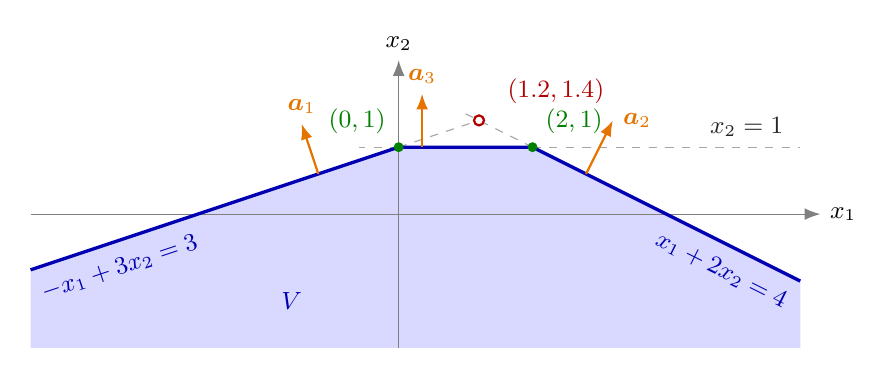
\begin{tikzpicture}[font=\small, >={Latex[length=2mm]}, x=0.85cm, y=0.85cm]
  \fill[blue!15] (-5.5,-0.8333) -- (0,1) -- (2,1) -- (6,-1) -- (6,-2) -- (-5.5,-2) -- cycle;
  \draw[gray, ->] (-5.5,0) -- (6.3,0) node[right, black] {$x_1$};
  \draw[gray, ->] (0,-2) -- (0,2.3) node[above, black] {$x_2$};
  \draw[gray!70, dashed] (0,1) -- (1.4,1.4667);
  \draw[gray!70, dashed] (2,1) -- (0.9,1.55);
  \draw[gray!70, dashed] (2,1) -- (6,1);
  \draw[gray!70, dashed] (0,1) -- (-0.6,1);
  \draw[blue!70!black, very thick] (-5.5,-0.8333) -- (0,1) -- (2,1) -- (6,-1);
  \draw[orange!90!black, thick, ->] (-1.2,0.6) -- (-1.45,1.35) node[anchor=south] {$\boldsymbol{a}_1$};
  \draw[orange!90!black, thick, ->] (2.8,0.6) -- (3.2,1.4) node[anchor=west] {$\boldsymbol{a}_2$};
  \draw[orange!90!black, thick, ->] (0.35,1) -- (0.35,1.8) node[anchor=south] {$\boldsymbol{a}_3$};
  \fill[green!50!black] (0,1) circle (1.8pt);
  \fill[green!50!black] (2,1) circle (1.8pt);
  \draw[red!70!black, thick, fill=white] (1.2,1.4) circle (1.8pt);
  \node[green!50!black, anchor=south east] at (-0.05,1.05) {$(0,1)$};
  \node[green!50!black, anchor=south west] at (2.05,1.05) {$(2,1)$};
  \node[red!70!black, anchor=south west] at (1.48,1.5) {$(1.2,1.4)$};
  \node[blue!70!black, anchor=north, rotate=18.43] at (-4.26,-0.53) {$-x_1+3x_2=3$};
  \node[blue!70!black, anchor=north, rotate=-26.57] at (4.95,-0.58) {$x_1+2x_2=4$};
  \node[gray!30!black, anchor=south] at (5.2,1.02) {$x_2=1$};
  \node[blue!70!black] at (-1.6,-1.3) {$V$};
\end{tikzpicture}
\end{document}
